\part{Introduction}


\chapter{Overview}

\begin{oopquote}
结构化程序设计基于任务的层次划分,而面向对象的设计则基于数据对象的层次划分。
\end{oopquote}

面向对象思想\cite{oop}诞生于20世纪60年代,并且最早被应用于Simula语言中,到20世纪80年代才真正引起计算领域的普遍关注。

在应用面向编程技术来进行开发时,类用来代表一组相似的对象(例如整数、链表等),通过类的继承可以形成树状结构,每个类实例的存储空间和行为自动地被其派生类使用,而且同一个类的多个实例对象能够执行相同的行为。

类可以看作是用来保存与一个对象相关的行为的存储仓库,而且在实践中可以将类组织成一个单根树状结构,称为继承层次。

在对象之间传递的消息是对特定行为的请求,并且伴随着完成这项任务所需的参数。

\begin{enumerate}
\item 任何事物都是一个对象。
\item 通过互相联系的对象请求其他对象执行一定的行为来完成计算。
\item 对象之间通过发送和接收消息进行通信。
\item 每个对象都有自己的存储空间来存储其他对象。
\item 每个对象都是一个类的实例。
\end{enumerate}


从最细微的问题到最复杂的项目,我们时刻在面对“软件危机”,即我们通过计算机来解决复杂任务的难度几乎总是要超出我们的实际能力。

在众多针对“软件危机”的解决方案中,面向对象编程是最近提出的一种方法。

使用面向对象技术有利于构建复杂的软件体系结构,但是面向对象编程是一种新的思考问题的方法,它着重于面向对象对于计算的含义,以及如何构建信息才能把我们的意图与其他人和机器进行顺利的交流,它更加要求优秀的程序员的天赋、创新、勤奋、逻辑思维、构建和提取抽象的能力以及经验。

充分有效地利用面向对象原则需要人们以一种新的方式来观察世界,但是,简单地应用一种面向对象语言本身并不能使我们成为一名真正的面向对象开发者。

使用面向对象语言只是会简化面向对象解决方案的开发,这并不代表掌握了面向对象思想,而且使用面向对象语言也可以开发面向过程的程序。


在人造的计算机语言中,语言与思维之间的关系比其在自然语言中表现得还要显著,也就是说,选择哪种程序设计语言来考虑待解决的问题,会影响或改变算法的设计。

\section{FORTRAN}


下面以基因研究中的一个问题来证明计算机语言和问题解决方案之间的关系。

在一项分析DNA序列的任务中,为了将任务简化,DNA可以用一个由N个整数组成的矢量来表示,其中N非常大(大约好几万)。我们的任务是判断DNA序列中是否包含重复的长度为M的序列片断,其中M为固定的数值常量(比如5或10)。


\begin{figure}[htbp]
\centering
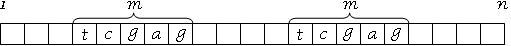
\includegraphics[scale=0.7]{dna-vector.png}
\caption{由N个整数组成的矢量来表示的DNA序列}
\label{fig:dna-vector}
\end{figure}

使用FORTRAN语言编写的解决这个问题的计算机程序如下:

\begin{lstlisting}[language=Fortran]
		DO 10 I = 1,N-M
		DO 10 J = 1,N-M
		FOUND = .TRUE
		DO 20 K = 1,M
	20	IF X[I+K-1] .NE. X[J+K-1] THEN FOUND = .FALSE
		IF FOUND THEN ...
	10	COUTINUE
\end{lstlisting}

\section{APL}


如果使用APL语言来编写这个问题的解决方案,需要重新考虑这个问题,把数据重新安排在一个N行M列的矩阵中,而不是前面所使用的由N个元素组成的矢量。

\begin{figure}[htbp]
\centering
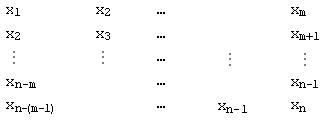
\includegraphics[scale=0.7]{dna-apl.png}
\caption{使用N行M列的矩阵表示DNA序列}
\label{fig:dna-apl}
\end{figure}

把矩阵按行排序(即把一行看作一个单元,在排序过程中移动整行)。如果有任何序列片断被重复,那么在排序后的矩阵中相邻的两行就会有相同的数值。

\begin{table}[htb]
\centering
\begin{tabular}{cccccc}
.&	.&	.&.	&.	&.	\\
T	&G	&G	&A	&C	&C\\
T	&G	&G	&A	&C	&C\\
.&	.&.	&.	&.	&.	\\
\end{tabular}
\end{table}


检查如何满足这项条件很容易。在这里,APL程序之所以快与APL语言本身无关,而是与算法有关。简单的讲,FORTRAN程序使用了一个$O(M\times N^2)$的算法,而APL程序使用的排序方案需要大约$O(M\times N\log N)$次操作。


上述示例的目的并不是说明APL语言在任何情况下,都比FORTRAN语言更有效,而是指APL程序员很自然地被引导发现一种完全不同的解决方式。

虽然使用APL语言很难写循环,而排序却很简单——作为语言组成部分,排序被定义为内部操作符。这样,由于排序运算很容易表达,APL程序员倾向于寻找关于它的创新性应用。这也就说明了解决问题的编程语言是如何引导程序员采用不同的思维方式来看待问题的。用来表达思想的语言可以影响或引导思维,这一点在程序设计语言方面得到了很好的体现。

Spair-Whorf假说认为存在这样一种情况:一个生活在某种特定语言环境下的人可能产生或者表达一些想法,这些想法无论如何也无法被生活在另外一种语言环境下的人所翻译和理解。根据假说提倡者的观点,这种现象可能发生的情况是:在后者的语言中没有对应的词汇或者缺少相关的概念来表达前者的想法。


\section{Turing Machine}

将人类语言产生上述这种现象的可能性与计算机科学中几乎直接对应的计算机语言产生这种现象的可能性相比较是一件有趣的事情——这就是丘奇猜想(Church’s Conjecture)。


逻辑学家Alonzo Church所发表的丘奇假说的内容是:
\begin{quote}
\emph{任何一种具有明确步骤的计算都可以通过图灵机来实现。}
\end{quote}





图灵机是一种可不受存储容量限制的假想计算机,但是图灵机本身是一种极其简单的装置,不需要有很多特性的某种语言来模拟这个装置。

如果我们接受丘奇猜想,那么任何可以模仿图灵机的语言都足以运算任何可实现的算法。为了解决这个问题,首先需要寻找能够生成所期待结果的图灵机。通过丘奇猜想可以知道这种图灵机一定存在,然后用我们所擅长的语言来模拟图灵机的运行。这样关于编程语言相对“能力”的讨论——如果我们把能力理解为“解决问题的能力”——是毫无意义的,而且我们也就陷入了Alan Perlis所提出的“图灵机泥潭”中,这种讨论既无意义又难以摆脱。



需要注意的是,丘奇猜想在某种意义上几乎与Spair-Whorf假说完全对立。


\begin{compactitem}
\item 丘奇猜想认为在基本方法上,所有的编程语言都是一样的。或者说,一种语言能够表达的想法,在理论上,用另一种语言也能表达。
\item Spair-Whorf假说则认为,存在这样一种可能,某些想法能用一种语言表达,却不能用另外一种语言表达。
\end{compactitem}


人们后来对自然语言提出了一种“图灵机-等价”理论,意思是说,只要通过充分的工作,任何想法都可以用任何语言来表达。

例如,一个一直生活在热带的人无法直觉地用自己的语言对不同类型或用途的雪进行分类,也无法判断雪域的范围,但是只要通过一定时间的培训,就一定能够掌握这种技能。

同样,面向对象技术也不能提供任何新的计算能力,使得原来通过其他方法在理论上无法解决的问题得到解决,但是面向对象技术确实提供了一种方式,使得解决问题更加容易和自然,而且这种方式有效地改善了大型软件项目的管理。


无论是计算机语言还是自然语言,语言只能引导思维,而不能阻止思维。面向对象编程不仅仅是在编程语言中加入一些新的特征,更重要的是,它是用来分析处理问题和开发计算机程序解决方案的一种崭新的思考方式。

可以肯定地说,一个由具有共同兴趣的个体组成的群体,倾向于发展他们自己的特殊词汇,一旦这些词汇形成,它们就会影响这些人的思维方式,而对于群体以外的人,这种方式很难理解,这本身就是一个OOP的实例。

既然面向对象思想在一定的原则下不需要面向对象语言就可以使用,那么面向对象术语的使用就能够帮助程序员以一种对于没有OOP术语的人来说也能理解的方式去思考问题。


\chapter{Real World}

下面首先考虑一下我们如何处理现实世界的情况,然后再去考虑在使用计算机解决问题时如何应用这种技术模式。

假设有一位名叫Chris的人想送花给他的一位叫Robin的朋友,Robin生活在另外一个城市。因为距离太远,Chris不能亲自把花送给他的朋友。不过,可以通过别的办法来完成。Chris来到附近的一家花店,这家花店由一个名叫Fred的花商经营。Chris把打算送给Robin的花的种类和Robin的地址告诉给Fred。这样Chris就可以确信他的花可以方便地送到他的朋友那里了。

\begin{figure}[htbp]
\centering
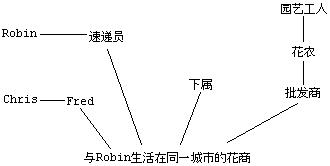
\includegraphics[scale=0.6]{flower.png}
\caption{现实世界中的实例}
\label{fig:flower}
\end{figure}

这里解决问题的方法就是找到一个合适的代理(也就是Fred),并且把自己的要求告诉他。代理有责任完成这些要求,Fred会选择某种方式——一种算法或一系列操作——来完成这项任务。Chris没有必要了解Fred使用什么方法来完成任务。实际上,使用代理的人通常不想了解完成任务的细节,这些细节一般都是隐蔽的。

通过调查可以发现,Fred向一位与Robin生活在同一城市的花商传递了一条信息,然后,那名花商可能会让一名下属来安排这件事。接着花和另外一条消息将交给一个速递员。这样依次进行下去。此时我们又会发现,与Robin生活在同一城市的那个花商一直都从花卉批发商那里购进花。同样地,花卉批发商又与花农交易,而花农则要管理园艺工人。

由此,我们得到关于通过面向对象思想解决问题的初步结论:解决问题需要很多其他个体的帮助。没有这些个体的帮助,问题难以解决。简单概括如下:

\begin{quote}
\emph{一个面向对象程序可以由一个团体(集合)组织而成,这个团体由一组互相作用但又松散连接的叫做“对象”的代理组成。每一个对象都扮演一个角色,对特定的任务负责,并且为团体中的其他成员提供特定的服务或者执行特定的行为。}
\end{quote}



\section{Message}

开始,Chris向花商Fred提出要求,此项要求导致了另外一项要求,然后又继续导致更多的要求,直到花最终送到Chris的朋友Robin手中。

通过这一系列的连锁反应,Chris的要求最终被实现了,而且由此可以看到,团体的成员通过传递要求来相互协作。

下面提出的通过面向对象思想解决问题的原则是确定传递工具来指示下一步行为。


在面向对象编程中,行为的启动是通过将“消息”传递给对此行为负责的代理(对象)来完成的。

消息对行为的要求进行编码,并且伴随着执行要求所需的附加信息(参数)来一起传递。“接收器”就是接收消息的对象。

如果接收器接收到了消息,那么同时它也接受了消息所包含的行为和责任,然后接收器响应消息,并执行相应的“方法”以实现要求。

与消息传递相关的是信息隐蔽原则——提出要求的客户不需要了解实现该要求的具体方式,还有另外一条原则——我们所知道的所有人都是隐藏在消息传递过程中的。客户如果要完成一项任务,首先的想法就是寻找能够执行这项任务的人。


面向对象编程的一个重要部分就是可复用组件的开发。使用可复用组件的第一步,也是非常重要的一步,就是程序员能够接受、信任他人编写的软件。在实际的计算机解决方案中,最终是通过对象的相互作用来完成计算的。

在传统的语言中,信息隐藏(information hiding)也是编程的一个重要方面。虽然根据要求两者都会运行一系列预定义的步骤,但是它们也有两点截然不同的地方。

\begin{description}
\item[首先] 每一条消息都与一个指定的接收器相对应,接收器就是接收消息的对象。过程调用却没有指定的接收器。
\item[其次] 消息的解释(即用于响应消息的方式)由接收器来决定,并且随着接收器的不同而不同。
\end{description}

例如,Chris给他的一位名叫Elizabeth的朋友发了一条消息,她接收到消息之后,立即采取了相应的行动(即把花送给了他们共同的朋友Robin)。但是,Elizabeth完成要求的方法和Fred完成相同要求的方法是完全不同的。

如果Chris让牙医Kenneth将花送给Robin,而Kenneth可能没有办法解决这一问题。如果他完全理解了这个要求,则有可能向Chris返回一个信息来说明错误。

从上述可以得出,消息传递与过程调用的区别是:消息传递有一个指定的接收器,解释——选择响应消息的方法——可能因接收器的不同而不同。通常,在程序运行之前,人们不会知道任何消息的接收器,也不会知道调用了哪些方法。

一般情况下,消息(函数或过程名称)和响应消息的代码段(方法)之间是后期绑定的关系。与之对应的是,传统过程调用中名称与代码段之间的早期(编译时或链接时)绑定关系。

\section{Responsibility}


面向对象编程的一个基本概念就是用责任来描述行为。例如,Chris对行为的要求仅仅表明他所期望的结果(把花送给Robin)。Fred可以任意选择使用的方法来实现所期待的目标,并且在此过程中不会受到Chris的干扰。

通过用责任来讨论问题,提高了问题抽象的水平,使得对象之间更加独立,这正是解决复杂问题的关键。通常用协议来描述与一个对象相关的所有责任的集合。

传统程序的执行通常是通过对数据结构进行操作——例如,改变数组或记录中的域。与此相反的是,面向对象程序则要求数据结构(即对象)提供服务。


从传统的、结构化数据的角度来观察软件与从面向对象的角度来观察软件之间的区别,可以得到下面的结论:

\begin{quote}
\emph{不要问你能为数据结构做什么}

\emph{要问数据结构能为你做什么}
\end{quote}

\section{Class}

Chris对Fred提出送花给Robin的要求之后,他大致上可以认定这个事件会发生在Fred的花店里。Chris做出这样的假定是基于以往同其他花商打交道的经验,因此Chris认为Fred作为这一类别中的一个实例,应该适用普遍的模式。

这里。我们可以用花商来代表所有花商中的一个类别(或者是类),从而可以把这些概念总结成面向对象编程的另外一个原则:

\begin{quote}
\emph{所有对象都是类的实例。在响应消息时调用何种方法由类的接收器来决定。}

\emph{一个特定类的所有对象使用相同的方法来响应相似的消息。}
\end{quote}

对象是对状态(数据值)和行为(操作)的封装,因此对象和专用计算机有很多相似之处。

\begin{compactitem}
\item 对象的行为由对象类来规定。
\item 每个对象都是某个类的一个实例。
\item 同一个类的所有实例都以相似的方式(即调用同一方法)来响应相似的要求。
\end{compactitem}





对象通过调用方法表现其行为(类似于执行一个过程),以此来响应消息。对消息(即所使用的特定的方法)的解释由对象决定,并且随着对象类的不同而不同。



\section{Inheritance}

Chris还有Fred更多的信息——这不仅是因为他是一个花商,更是因为他是一个店主。例如,Chris知道钱的转移是这项交易的一部分,同时作为付款的凭证,Fred交给Chris一张收据,而这些行为同样也会发生在食品商、文具商和其他店主身上。由此可知,花商这个类别是店主类别的一个特殊类别。Chris知道,关于店主的一切对于花商也同样适用,于是这也适用于Fred。

下面将讨论Chris是如何组织关于Fred的信息的,我们可以通过分类层次来考虑。Fred是一个花商,而花商又是店主的一种特殊形式。进一步讲,店主是一个人。而Chris知道所有关于人的一切也同样适用于Fred,尽管这些信息没有直接与他发生联系。


一般类别的信息也适用于特殊类别,这样的原则称为继承。通常都利用一种交错的图像技术来说明这种关系,尤其是当很多个体有不同的归属时。使用这种技术可以把类组成树状层次结构。在这种结构中,比较抽象的类位于树的顶端,比较具体的个体位于树的底部。


类可以组织成一个有层次的继承结构。一个子类继承层次树中更高一层的父类的属性。抽象父类是指没有具体实例的类,它只是用来产生子类。通过继承,树中较低层次的类,可以存取和使用与树中较高层次的类相关的数据和行为。


\section{Override}

为了解决类的层次结构中平行类的相关问题,需要寻找一种技术,能够处理一般规则以外的特例。

我们可以通过在子类中发布一条信息来解决此问题,这条信息可以改写(override)从父类继承的信息。通常,给子类中某一方法取一个与父类中某一方法相同的名称,再结合寻找方法的规则(当响应特定信息时)来实现这个目的。

接收器类搜索并执行相应的方法以响应给定的消息。如果没有找到匹配的方法,搜索就会传导到此类的父类。搜索会在父类链上一直进行下去,直到找到匹配的方法,或者直到父类链结束。如果是前一种情况,就会执行方法;对于后一种情况,会产生错误信息。如果能在更高类层次找到相同名称的方法,所执行的方法就称为改写了继承的行为。

虽然编译器在运行时不能确定调用哪个方法,但是许多面向编程语言能够确定是否有合适的方法以供调用,并且能够产生错误信息作为编译时错误诊断,而不是运行时信息。

不同的对象都会对类的消息做出相应的反应,但执行的方法却不同,这也就是多态(polymorphism)的一种表现。



\chapter{Metaphor}



计算机执行程序的行为的模型是一个过程状态或者鸽子窝模型,或者说,计算机是一个数据管理员,跟随着一些指令模式,在存储器中从不同的槽(内存地址)中取出数值,用某种方式对它们进行转换,再将结果推入到另外的槽中。检查槽中的数值就可以确定机器的状态或者计算的结果。虽然这个模型与实际计算机内部的工作流程大致吻合,但对于我们理解如何使用计算机来解决问题,却没有多少帮助,而且这也不是我们大多数人解决问题的方式。

在面向对象框架中,我们几乎不提内存地址、变量、赋值或者任何传统编程术语,而只是使用对象、消息和某种行为的责任。

在面向对象编程思想中,用户拥有的是一组行为规范的对象,各个对象之间通过礼貌地交互来实现各自的愿望。


在很多方面,把编程比作创建“域”的观点和一种称为“离散事件驱动模拟”的计算机模拟很相似。简而言之,在离散事件驱动模拟过程中,用户为不同的模拟元素创建其计算机模型,通过模型来描述元素之间如何相互作用,并使它们运作起来。这几乎等同于通常的面向对象程序。

在通常的面向对象程序中,用户需要描述域中的不同实体代表什么、它们如何相互作用以及如何使它们最终运作起来。因此,我们可以得到这样的结论,也就是说,在面向对象编程中,计算就是模拟。


通过类和模拟的概念,初学者很容易理解隐喻(metaphor),隐喻有利于面向对象技术的应用,但是通常它却很容易被忽略。当程序员根据对象的行为和责任思考问题时,可以为程序员带来很多的关于日常经验的直觉、思想和理解力。当把问题想象成鸽子窝、邮箱或者包含数值的槽时,程序员几乎不需要什么背景知识就可以深入了解问题并对其结构化。这些都是隐喻的强大的解释力量的反映。

不同于以往的编程方法,使用面向对象编程思想分析问题和编写程序解决问题时,为开发者提供了更大的构件,开发者通过迅速地用它们组装自己的软件就可以解决问题,这一方面可以类比Lego玩具提供的各种组件。

通过减少软件组件之间的相关性,面向对象编程可以实现可复用软件系统的开发。这样的组件与软件应用的其他部分是隔离的,可以作为独立的单元来创建和测试。


可复用的软件组件允许程序员在更高的抽象层次上处理问题。我们可以简单地通过能被对象所理解的消息和对象需要执行的任务来定义和操作对象,而不必考虑执行细节。

当然,对象不可能总是通过礼貌地请求另一个对象执行某种行为来响应消息。如果这样,结果会形成一个无限的请求循环,就像两个绅士都礼貌地等待另一位先进门,或者像一个使用纸上签字的官僚机构,每一个人都把所有的待签纸传给组织中的另外的人。在某种程度上,至少有几个对象,除了传递请求给其他代理之外,还执行一定的工作。根据所使用的面向对象语言的不同,这项工作的完成情况也不同。

\begin{compactitem}
\item 面向对象/命令的混合语言(如C++语言、Object Pascal语言和Objective-C语言)通过基础(非面向对象)语言编写的方法来完成。

\item 更加纯粹的面向对象语言(例如Smalltalk或者Java)是通过语言基本体系结构所提供的“原始的”或者“固有的”运算指令来完成。

\end{compactitem}

另外,Peter Wegner提出了区别基于对象语言和面向对象语言的不同之处的方法,基于对象语言只支持抽象(如Ada),而面向对象语言还必须支持继承。

Apple Object Pascal语言最初是由Larry Tesler定义的,而Borland Pascal语言的最终演化成了Delphi语言。Objective-C语言的创建者是Brad Cox,在它作为C语言的扩展语言产生的同时,C++语言也开发完成,Smalltalk语言也有其公共流行版本Squeak。

\chapter{Abstraction}

在打开一本地图册时,首先会看到一张世界地图。这张地图只会显示某些最重要的特征,例如,各种山脉、河流和其他一些非常大的建筑物,而一些细小的特征都被忽略了。

随后的地图会描绘出一些小的地理区域,通常还有更多的细节。例如,一个洲的地图可能包括政治边界和一些主要的城市;一张关于更小区域的地图,例如一个国家,可能包括城市、乡村和更小的地理特征,比如某个山脉的名称;一张大城市的地图可能包括出入城市的主要道路;比城市更小的区域地图甚至可能标注出每一座建筑。

在每一级别水平上都会包括某些特定的信息,而故意忽略了某些其他的信息。当以更高级别的抽象来看待一件制品时,没有什么方法能够描述它的细节。而且,即使能够描述出这些细节(比如用极小的字),人们也无法吸收或处理如此大量的信息,因此,一些细节就这样简单地被忽略了。通常,人们只使用几种简单的工具去创建、理解和管理复杂的系统。抽象就是最重要的技术之一。


抽象是指对于一个过程或者一件制品的某些细节的有目的的隐藏,以便把其他方面、细节或者结构表达得更加清楚。通过抽象,我们可以建立起针对实际系统的不同层次的模型。在形成抽象或模型时,我们有意识地避免理解很多细节,而是集中精力在几个主要特征上面。我们经常用另外一个术语来描述这样的行为:信息隐藏。


信息隐藏描述了部分抽象,通过它,我们就可以有意地忽略某些特征,以便于能够集中强调其他特征。


\section{Abstraction Level}


在一个典型的面向对象程序中,有很多抽象层次。更高层次的抽象体现了面向对象程序的特征。在最高层次的抽象层次上,程序被看作是一个由很多对象组成的“团体”,为了实现共同目标,这些对象之间需要相互合作。


\begin{figure}[htbp]
\centering
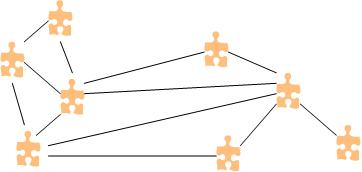
\includegraphics[scale=0.6]{abstract-level.png}
\caption{抽象层次}
\label{fig:abstract-level}
\end{figure}


在面向对象开发中,团体这个概念有两种不同的形式。第一,程序员团体,在现实世界中,为了完成应用程序,程序员之间必须互相合作。第二,程序员创建的对象团体,在虚拟世界里,为了实现共同目标,对象之间必须互相合作。而信息隐藏和抽象等面向对象思想对这两种形式都适用。

团体中的每一个对象都为组织中的其他成员提供服务。在这个最高级别的抽象层次上,需要强调的最重要的特征就是交流和合作的通道,以及成员之间相互合作的方式。

下一个级别的抽象不会在所有的面向对象程序中出现,也不被所有的面向对象语言所支持。但是,很多语言都允许一组对象一起工作,形成一个单元(unit)。关于这个思想的实例有Java语言中的包(packages)、C++语言中的名称空间(name spaces)和Delphi语言中的单元(units)。这种单元允许某些特定的名称暴露在单元以外,而其他的特征隐藏在单元内部。

单元这个概念继承了C和Modula等语言中的模块思想(module),面向对象编程思想应归功于早期的模块研究。

下两个级别的抽象是用来处理两个独立对象之间的交互。我们常说的是一个对象能够为其他对象提供服务。这种直觉的建立来自于对客户和服务器之间通信的描述。
这里的服务器只是表示提供服务的对象。这两个层次的抽象涉及了对这种关系的两种视角,一种来自于客户端,一种来自于服务器端。


在一个优秀的面向对象设计中,我们可以描述和讨论服务器所提供的服务,而无需提及客户在使用这些服务时可能执行的任何行为。可以把这想象成广告牌。


\begin{figure}[htbp]
\centering
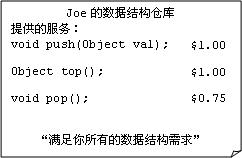
\includegraphics[scale=0.6]{ad-board.png}
\caption{广告牌}
\label{fig:ad-board}
\end{figure}

这个广告牌描述了一个数据结构(如堆栈)所提供的服务。这个级别的抽象通常用接口来表示,接口是一个与类相似的结构,它定义了行为,但不描述如何来实现这些行为:

\begin{lstlisting}[language=Java]
interface Stack{
	public void push(Object val);
	public Object top()	throws EmptyStackException;
	public void pop()	throws EmptyStackException;
}
\end{lstlisting}


下一抽象层次查看同一边界,但却不同于服务器端。这一抽象层次需要考虑抽象行为的具体实现。例如,有很多数据结构可以用来满足堆栈的要求。这一层次主要关注服务的具体实现方式。

\begin{lstlisting}[language=Java]
public class LinkedList implements Stack ...{
	public void pop()	throws EmptyStackException{...}
	...
}
\end{lstlisting}


在抽象的最底层需要单独考虑一项独立的任务,即一个方法。这一层次的抽象主要关注的是执行这一活动所需操作的精确顺序。例如,我们可能需要研究这样的技术,用来移走放入堆栈里的最近元素。

\begin{lstlisting}[language=Java]
public class LinkedList implements Stack ...{
	...
	public void pop() throws EmptyStackException{
		if(IsEmpty())
			throw new EmptyStackException();
		removeFirst();//delete first element of list
	}
	...	
}
\end{lstlisting}

在软件的开发过程中,每一个抽象层次在某些方面都很重要。实际上,需求经常要求程序员在各种抽象层次之间迅速地移动,也就要求我们在每一个抽象层次上执行相应的面向对象的分析。

在软件开发的早期,一个关键的问题就是如何确定正确的抽象级别。通常出现的错误是在低层次的抽象级别上反复思考,担心各种关键组件的实现细节,而不是努力地思考如何实现高级别的抽象,以促进有关问题之间的完全分离。

在软件开发过程中的任何时刻,程序员(或开发一个比较大的项目的设计小组)都必须进行缜密的思考,才能确定正确的抽象级别。对于特定问题,人们通常不愿忽略或者放弃很多的细节,但是实际上人们不能过多地关注细节,否则,一些重要的问题就会被掩盖掉。


\section{Abstraction Pattern}

抽象可以用来帮助理解复杂的系统。在某种程度上,抽象是系统结构的版图。我们所使用的结构可以反映出系统某些真实的方面,或者它可能只是一种思维的抽象,用来帮助我们理解真正的问题。

抽象的思想可以进一步划分为不同的形式。通常的技术是将一个层次划分成各种组成部分,当我们描述汽车是由发动机、传动装置、车体和车轮组成时,所使用的正是这个方法。

下一个理解层次是通过依次检查每一个组成部分来实现,这不过是分而治之(divide and conquer,分治法)的一个体现。

\begin{figure}[htbp]
\centering
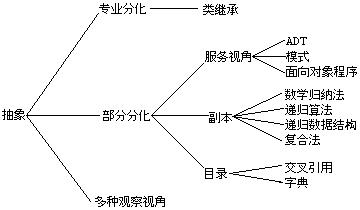
\includegraphics[scale=0.6]{abstract-pattern.png}
\caption{抽象的其他形式}
\label{fig:abstract-pattern}
\end{figure}

有时候我们使用不同类型的抽象。另外一种形式就是特化分层思想。对于汽车的理解就可以部分基于以下知识,首先,它是一个有轮子的车辆,其次,它是一种交通运输工具。另外我们还了解其他一些关于有轮车辆的知识,这些知识既适用于汽车,也适用于自行车。而且我们还了解其他各种不同的运输工具,同样地,这些知识也适用于驮马,也适用于自行车。面向对象编程语言广泛地使用这种抽象形式。

\begin{figure}[htbp]
\centering
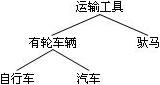
\includegraphics[scale=0.6]{abstract-example.png}
\caption{特化分层}
\label{fig:abstract-example}
\end{figure}

部分分化和专业分化的思想代表了在面向对象编程中使用的两种最重要的抽象形式,即通常所说的“是抽象”和“有抽象”。

\begin{description}
\item[是抽象]

专业分化是指“是抽象”,自行车“是有轮车辆”,它“又是运输工具”。

\item[有抽象]

部分分化就是“有抽象”,这一术语的含义很容易理解,例如汽车“有发动机”。
\end{description}

在实际的计算机程序设计过程中,“是抽象”和“有抽象”会与特定编程语言的特征联系在一起。

人们最常使用的用来帮助理解复杂系统的技术就是把抽象和分化成的各种组成部分结合起来。我们对汽车的描述就是一个这样的例子。理解下一个层次需要通过对每一个组成部分进行更精细的细节分析来实现。例如,对汽车发动机更精细一些的描述,就是把它看作圆柱体的组合,每一部分都能将燃料的爆炸转变成垂直方向的运动,并通过曲轴将圆柱体的上下运动转换成旋转运动。

另外一个例子是关于如何组织人体运动的信息。在某一层次上,我们只关系各种组织,把人体看作是由骨骼(保持刚性)、肌肉(产生运动)、眼镜和耳朵(产生感觉)、神经系统(传递信息)和皮肤(把各个部分连接起来)组成的。在下一个抽象层次上,我们可能会考虑肌肉是如何工作的,并且会考虑一些比如细胞结构和化学作用的问题,而化学作用又是由分子结构决定的。为了了解分子,又得把分子继续分解为原子。

任何解释都必须基于正确的抽象层次来阐述。如果试图以原子层次的细节来解释一个人是如何行走的,将会是极其困难的。


\section{Encapsulation}


创建一个大系统的关键步骤就是将其分成合理的组成部分。不管是编写软件还是建造汽车,通过将整体的大的系统进行合理的划分,就可以分配人员基本独立地进行各部分的工作。

使用封装这个术语是指内部视角和外部视角之间有着严格的区分,因此制造发动机的小组成员对传动装置只需要有一个抽象的(也就是外部的)理解,而制造传动装置的小组成员则需要对传动装置具备详细的内部理解。

封装的一大优点在于允许我们考虑实现互换的可能性。当我们把一个系统划分为几个部分时,理想的目标就是将各个部分之间的相互作用减少到最少。例如,通过封装发动机的行为,可以使其与传动装置隔离,我们可以把一种类型的发动机转换成另外的类型,而不会影响系统其他部分的运行。

为了将这些思想应用于软件系统,我们需要一种方式来讨论软件组件执行的任务,而且这种方式要和组件满足责任的方式区别开来。


\section{Interface}

在软件系统中,我们使用接口和实现这两个术语来描述一项任务包含哪些内容和如何实现任务,以及外部视角和内部视角之间的区别。

接口描述系统被设计用来做什么,这是抽象使用者必须理解的思想。接口并没有说明所分配的任务应如何执行。因此,接口通过与完成抽象的实现相匹配来使系统正常工作。在汽车工业中,发动机的设计者会与传动装置的接口相联系,而传动装置的设计者必须实现这些接口。同样,开发复杂的计算机软件系统的一个重要步骤就是将一项任务分成几个部分。这些部分可以由小组的不同成员来开发。每一个部分都有两个方面:接口显示给外部世界,而实现用来完成接口的要求。

接口和实现的分离不但使得在较高层次上理解一项设计更加容易(因为接口的描述比任何特定实现的描述都简单得多),而且使软件组件的互换性成为可能(因为可以使用任何实现,只要它能够满足接口规范)。

当一个系统中组件的数量越来越多的时候,以“目录”的方式来组织它们通常是很有效的。

在日常生活中我们要使用很多不同形式的目录。例如,电话号码簿、字典或搜索引擎等。类似地,在软件中也使用各种各样的目录。一份关于系统中所有类的简单列表就是一个这方面的例子。

另外一个目录的例子就是由类所定义的所有方法组成的清单。Java标准库的类参考手册就是一个非常有用的目录。

以上的每一个实例都体现了以下思想,目录为用户提供了一种机制,使用户可以从一个范围很大的集合中迅速地定位到某一特定的位置(可以是类、对象或者方法)。


接口描述了软件组件所提供的服务,却不必描述完成服务所使用的技术,这个思想是理解和处理复杂软件系统的核心手段。在上述关于送花的实例中,强调的也是这种抽象。这个实例的最后结果是有很多人都参与了送花的过程,并且在每个流程都各司其职。

\begin{figure}[htbp]
\centering
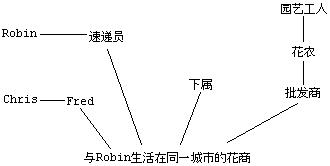
\includegraphics[scale=0.6]{interface-service.png}
\caption{服务视角}
\label{fig:interface-service}
\end{figure}


团体中的每个成员为这个团体中的其他人提供服务,没有一个成员能够自己独立地解决问题,只有通过互相协作,才能实现所期待的结果。


服务提供者(service provider)的概念在开发复杂软件系统时是非常有用的。软件组件为和它相互作用的其他组件提供服务。在现实生活中,我们经常通过成员提供的服务来刻画团队成员的特征(速递员负责把花从花商那里送到顾客手上),因此,这一比喻可以让我们用日常生活中思考问题的方式来考虑一个大规模软件系统。



\section{Compounding}


复合法是另外一种从独立的部分创建复杂结构的强大技术。这一思想从少量几个基本的形式开始,然后增加一些规则,将各个形式结合起来创建新的形式。复合法的主要原则是允许合并机制,既可以作用于新形式也可以用在原来的基本形式上。

正则表达式(regular expression)充分地说明了这项技术。正则表达式是描述一系列数值的简单技术,它的描述是从确认基础的字符表开始的,例如,字符a、b、c和d。任何单独字符的例子都是一个正则表达式。下一步,我们增加一条规则,即由两个正则表达式组成的复合结构也是一个正则表达式。通过反复地应用这一规则,就可以发现,任何有限的由字符组成的字符串都是正则表达式。

\begin{lstlisting}[language=bash]
abaccaba
\end{lstlisting}

下一个合并规则是说两个正则表达式的可替换形式(用竖线“|”来表示)是一个正则表达式。正则表达式遵循这样的运算规则,复合运算优先于可替换运算规则,因此,下面的模式代表一系列由三个字母组成的值,由ab开始,以a、c或者d结束。

\begin{lstlisting}[language=bash]
aba|abc|abd
\end{lstlisting}

可以用括号来表示分组,因此还可以表示成下面的形式:

\begin{lstlisting}[language=bash]
ab(a|c|d)
\end{lstlisting}


最后,符号“*”(通常称为星号)用来表示“0或者多个重复”的概念,把这些规则结合起来,就可以描述非常复杂的字母组合。例如,下面一系列字符值的描述是以a或者b的循环紧接着一个c来开始,或者是以dd两个字母序列开始,然后是字母a。

\begin{lstlisting}[language=bash]
(((a|b)*c)|dd)a
\end{lstlisting}

复合法的思想也是类型系统的基础。类型系统开始于一些原始类型,如整数类型和布尔类型。类的思想允许用户创建新的类型,这些新的类型可以包含从前一类型构建出的数据字段,这里的前一类型可能是原始类型,也可能是用户自定义的数据类型。既然可以以先前所定义的类为基础来创建类,那么就可以逐渐地构建非常复杂的系统。


\begin{lstlisting}[language=Java]
class Box{//a box is a new data type
	...
	private int value;//built out of the existing type int
}
\end{lstlisting}



复合法原则还有另外一项应用,就是便于进行窗口布局的用户界面控件库。窗口是由一些简单的数据类型组成的,如按钮、滑块和绘图板。各种类型的布局管理器都要创建一些简单的结构。例如,一个网格布局定义了一个矩形网格,每个网格的大小相同,边界布局管理器确定了这样一种规范,允许5个组件分布在屏幕的北、南、东、西和中各个部位。

和正则表达式一样,重要的是这一窗口也可以作为其他窗口的一部分。例如,如果我们要定义一个窗口,左边有3个滑块,中间有一个绘图板,16个按钮4个一组地依次排列在右边,文本框排列于顶部。我们通过把简单的窗口放置在较为复杂的窗口中,就能够实现这一需求。


\begin{figure}[htbp]
\centering
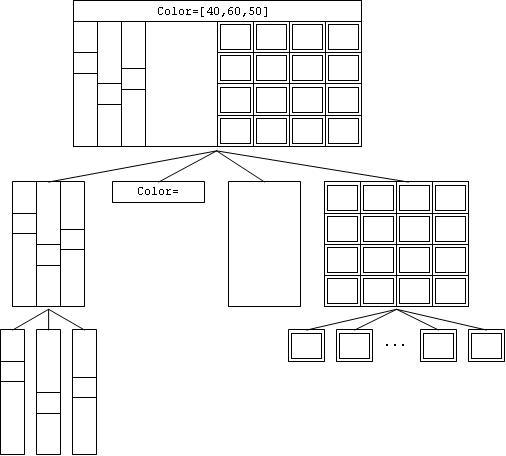
\includegraphics[scale=0.5]{compound-window.png}
\caption{复合窗口}
\label{fig:compound-window}
\end{figure}

大多数计算机程序本身就可以看成是复合的产品,这时,方法或者过程的调用就是复合的机制。我们从语言的基本语句开始(赋值等),通过这些可以建议一个实用的函数库。以这些函数库为基础,就可以形成更加复杂的函数。如此继续下去,每一层都建立在上一层的基础之上,直到最终完成所要求的应用程序。

抽象通常与组件(component)划分相联系,组件封装了某种主要特征,并通过简单和固定的接口(interface)与其他组件相互作用。组件的划分意味着我们可以把一项大任务分成一个个的小问题,这样这些小问题就可以大体上相对独立地进行解决。提供符合接口要求的实现(implementation)是每一个组件开发者的责任。



另外一个处理复杂问题的方法是使用特化分层来构建抽象,有时也把它称为分类系统。例如,在生物学上把生物分为动物和植物,动物又分为脊椎动物和无脊椎动物,脊椎动物包括哺乳动物,哺乳动物包括狗、马、鲸鱼等。

但是这种分类同时也存在特例,鸭嘴兽是产蛋的哺乳动物,因此,如果我们把这种特殊现象与哺乳动物生产幼仔来繁衍后代的特征相联系,就需要更改鸭嘴兽的特征,来解释为什么鸭嘴兽属于哺乳动物,却能够产蛋的事实。

面向对象语言也需要一种机制,来改写从更加普遍的类别继承而来的信息,这就需要更加深入地讨论类继承的思想。

使用特化分层抽象与以前的抽象之间的主要区别在于越特化的抽象层次是越普遍化的抽象层次的表现。但是这与前面所使用的从肌肉的特性抽象到各种化学作用的描述时的观点是不同的。这两种不同的关系可以描述成是(is-a)继承关系和有(has-a)继承关系。

然而实际上,使用任何一种抽象类型的原因都是一样的。抽象的原则允许我们忽略某些细节,以便更易于表现少数几个主要的特征。同样的技术也应用在面向对象语言。新的接口从现有的接口上形成。一个类从已有的类那里继承而来,这时,和原始类相关的所有特性(数据字段和行为)都同样适用于新类。

在讨论Java AWT(Abstract Windowing Toolkit)库的案例中,当使用AWT创建一个新的应用程序时,主类作为Frame的子类,依次地和AWT库的其他类链接。Frame是应用程序窗口的一种特殊类型,但是它也是Window类的一种更特殊的形式。Window可以包括其他的图形对象,因此它也是一个Container类型。每一个继承层次都为更低的层次提供方法,即使最简单的应用也需要使用如下的方法。

\begin{table}[htbp]
\centering
\begin{tabular}{ll}
setTitle(string)	&从类Frame继承而来\\
setSize(int,int)	&从类Component继承而来\\
show()			&从类Window继承而来\\
repaint()			&从类Component继承而来\\
paint()			&从类Component继承而来,将在新的应用程序中被改写\\
\end{tabular}
\end{table}

\begin{figure}[htbp]
\centering
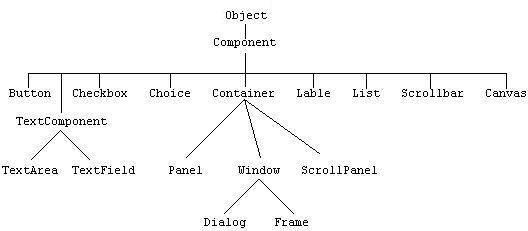
\includegraphics[scale=0.5]{awt-example.png}
\caption{Java AWT}
\label{fig:java-awt-example}
\end{figure}

另外一种形式的抽象就是分类系统——在面向对象语言中更倾向于使用继承层次(inheritance hierarchy)这个术语。这里,层次是一个普通类别的更详细的表示。一个这种类型系统的例子就是生物学上的分类。每一层次都是上一层次更加特殊的表现。这种分类可以简化理解,因为更一般层次的知识适用于那些更特殊层次的对象。当这项技术用于软件系统时,它也简化了新组件的创建,因为新组件和已有的类别相关,新组件可以自由地利用已有类别的所有功能,例如Java类库中的Frame组件。


\chapter{Pattern}

当面对一个新问题时,大多数人会首先看一看他们曾经解决过的问题和现在的新任务有什么共同的特征。那些原来的问题可以作为一种模式,新问题也将以相似的方式进行处理,只需针对不同的环境做一些必需的改动。

这一观察结果暗示了软件模式的思想。模式就是试图为问题提出一个已经被证实的解决方案,以便于能够很容易地用类似的方式来解决以后的问题。在面向对象领域,这一思想广泛地用来描述对象团体中成员之间的相互作用模式。

下面的用一个简单的例子证明模式的这一思想。假设正在开发一个网络应用程序。这意味着应用程序的一部分运行于一台计算机,另一部分运行于通过网络连接着的另外一台计算机。在这两台计算机之间建立实际的连接和通过连接传递信息这些细节,可能与应用程序的大部分应用都毫不相关。构建这些关系的一种方式就是使用一种称为代理的模式。代理是一种将网络连接隐藏于其中的中介。对象可以和代理相互作用,但却完全感觉不到代理内部使用哪种具体的网络连接类型。当代理接收到一项关于数据或者行为的请求时,它把这些请求打成一个包,通过网络进行传输,然后接收到响应包,解包,再将响应信息返回给客户。如下图所示,通过这种模式完成客户请求,客户完全感觉不到网络协议的细节。
\[\mbox{客户}\longrightarrow \mbox{代理} \longrightarrow \mbox{服务器}\]

需要注意的是,这种模式的描述是如何抓住交互的关键点(对客户隐藏通信协议的需要),而忽略交互的其他方面的(例如,在客户和服务器之间传递的特定的信息)。

模式是对某些已经在多个地方、以多种形式出现过的问题的解决方案的概括性的描述。模式描述了如何确定问题,同时解释采用某种解决方案和考虑其他替代方法的原因。
在某种程度上,一个对象就是一个简单的抽象数据类型。实际上,一个对象定义就是一个抽象数据类型,但是,面向对象编程的概念是建立在抽象数据类型思想上的,并且增加了代码共享和代码可复用性这一重要的创新。

汇编语言和过程作为抽象机制把程序员的视角集中在功能层次上:如何完成一项任务。而随着程序开发逐渐向模块和ADT的延伸,计算则从以功能为中心转变为以数据为中心,在这里,数据的重要性在于它们的结构、表示和操纵。

面向对象编程从以数据为中心的角度来看待世界的观点开始,继续向前发展。不是数据抽象本身对计算重要,ADT才是有用的抽象,因为它可以用服务(service)来定义,并且提供给程序的其他部分。其他类型的抽象也可以用类似的方法进行定义,不是根据它们特定的行为或者数据值,而是根据它们所提供的服务。

\begin{description}
\item[汇编语言]
\item[函数和过程]	

以功能为中心的观点
\item[模块]
\item[抽象数据类型]

以数据为中心的观点
\item[面向对象编程]

以服务为中心的观点
\end{description}

关于如何构建一个计算机程序的观点从以功能为中心开始,发展到以数据为中心,最后以服务为中心。这样,面向对象编程代表了这一发展过程的第3步。

除了计算以服务为中心的观点外,面向对象编程还在抽象数据类型的概念上增加了几个重要的新的思想。其中最重要的就是消息传递(message passing)。活动是通过对特定对象的请求(request)初始化的,而不是通过对特定功能的调用初始化的。


隐藏在消息传递中的思想是消息的解释(interpretation)可以随着对象的不同而改变,即消息所导致的行为和响应依赖于接收信息的对象。这样,push对于堆栈是一个含义,但对于机械式手臂控制器却是另一个完全不同的含义。因此操作的名称不需要惟一,使用简单而直接的命名形式有助于创建更容易阅读和理解的代码。

最后,面向对象编程还增加了继承(inheritance)机制和多态(polymorphism)机制。继承允许不同的数据类型共享同一代码,这将减少代码的数量,并且增加代码的功能。多态允许这些共享代码被定制成适合某一数据类型的特定环境。对于组件独立性的强调有助于软件的增量开发,在这一过程中,每个软件单元在合并成一个大系统之前,都可以独立地进行设计、编码和测试。

面向对象设计不同于传统的软件设计,它的驱动力是对不同软件组件分配责任。如果没有主体去执行动作,就不会有行为发生,因此每一个行为都必须指定给对象集合的某个成员。反之,对象集合中成员完成的行为要能够实现所期待的目标。






















